\chapter{Conclusion and Further Work}\label{ch:conclusion}
\def \path {other/}
\def \imgpath {\path/images}

In this thesis, we have examined the effectiveness of using complex wavelets as
basis functions for deep learning models. We summarize the key results we have
found before describing possible future extensions of our work. Some of these
are natural expansions which we were not able to explore due to time constraints, and some
are propositions for tying together interesting pieces of work that were developed
towards the end of the project.

% We first looked at ScatterNets, a type
% of feature extractor that builds invariances using the complex magnitude
% operation, demodulating image energy towards zero. Having examined the
% properties of these ScThen we looked at a method
% that does not rely on demodulation, and simply learns complex gains for wavelet
% subbands. The input channels could then be mixed in a learned way much like a
% regular CNN convolutional layer. The first part of our research looked
% at ScatterNets as they were a promising starting point for achieving this task.

\section{Summary of Key Results}
\textbf{\Autoref{Chapter}{ch:dtcwt_scat}} shows how using the separable spatial implementation of
the $\DTCWT$ as the chosen wavelets for the original ScatterNet design greatly
speeds up computation compared with Fourier domain implementations of complex
wavelets (see \autoref{tab:ch3:scat_speeds}). We
derived the backpropagation equations for wavelet and scattering layers, aiding
the use of ScatterNets as part of deep networks (this was crucial for our work
of \autoref{ch:invariant}). As part of this, we tested
the performance of the $\DTCWT$-based ScatterNet as a front end to a simple CNN for
some small classification tasks, comparing its performance to a Morlet based system. We
found that as well as being faster, the performance was often better when using
the $\DTCWT$ wavelets \autoref{tab:ch3:comparison}. When doing these tests, we
found that of the wavelet choices available for the $\DTCWT$, those with the
fewest taps (and hence wider transition bands and worse stopband rejection)
performed the best. This is somewhat surprising and while we were not able to
investigate why due to time constraints, it may provide some interesting
insights as to what the CNN backend is doing. It also may have been a side
effect of the small image sizes used in the classification task.

\textbf{\Autoref{Chapter}{ch:visualizing}} builds a visualization tool we call the
DeScatterNet. We use this to interrogate the input patches that most highly
excite the ScatterNet outputs on a subset of images from ImageNet (see
\autoref{fig:ch4:reconstructions}). We saw that
the second-order scattering coefficients are most highly excited by ripple and
checkerboard-like patterns. These were very different to the patterns
that most highly excite filters of a CNN. We believe this may explain why
ScatterNets perform well on texture discrimination \cite{bruna_invariant_2013}
but less well on natural image classification \cite{oyallon_deep_2015}. We then
performed some occlusion tests on a hybrid network with a ScatterNet front end
and CNN backend and saw that the CNN was able to operate with little degradation when the 
second-order scattering coefficients were zeroed out (there was only a small drop in
classification accuracy), but it suffered greatly when the zeroth or first-order
coefficients were removed. We also found the surprising result that on the
datasets we tested, the filters with diagonal edges were less important than their vertical or
horizontal counterparts (\autoref{fig:ch4:occlusion1}). If the input images were
rotated by $\pm 30\degs$ then the diagonal channels became the most important.
This echoes the experiments of
\citeauthor{blakemore_development_1970}\cite{blakemore_development_1970} who
controlled the orientation of edges exposed to kittens in their development
stage. Finally, this chapter showed some ways to expand on the ScatterNet
network and shows the features possible with these extensions in \autoref{fig:ch4:newshapes}.
This last section inspires the work of \autoref{ch:invariant}
and \autoref{ch:freqlearn}.

\textbf{\Autoref{Chapter}{ch:invariant}} reworks the ScatterNet into individual layers.
This redesign allows us to rethink how we want to use wavelets, and we introduce
the \emph{learnable ScatterNet} made up of \emph{locally invariant convolutional
layers}. Rather than applying the same layer twice to get a second order
ScatterNet, we introduce mixing across the output channels, taken after the
magnitude operation. The flexibility of the proposed layer means it can be used
in a ScatterNet-like system, where the number of output channels grows
exponentially with the number of layers, or in a CNN-like system, where the
number of output channels remains mostly constant across layers. We experimented
with both possibilities, showing that the extra learnability definitely helps
the ScatterNet style system (\autoref{tab:ch5:hybrid_scat}) and CNN style
networks (\autoref{fig:ch5:inv_results}). The demodulation of energy from the complex
modulus means that the proposed locally invariant layer can only be used a few
times. In particular, we saw that the layer performed best when used where a CNN
would naturally downsample (or pool) the input.

\textbf{\Autoref{Chapter}{ch:freqlearn}} looks at learning in the wavelet space without
taking complex magnitudes. We present the wavelet \emph{gain layer} which takes
inputs to the wavelet domain, learns complex gains to attenuate/accentuate
different subbands, mixes the subbands across the different channels and offers
the ability to return to the pixel domain with the inverse wavelet transform.
Our experiments have been promising but are still only preliminary. We
show that the \emph{gain layer} can learn in an end-to-end system, achieving nearly
the same accuracies on CIFAR-10, CIFAR-100 and Tiny ImageNet to a reference system with
only convolutional layers (\autoref{fig:ch6:gl_results}).
Despite the slight reduction in performance, we saw some
nice properties of the gain layer. The bandpass gains were very sparse,
needing very few non-zero coefficients and visualizations of what the layers
were responding to showed that the gain layer had nice
spatial roll-off properties (\autoref{fig:ch6:visualizations}).
We then found using a ReLU on the lowpass coefficients, and
Batch Normalization and a ReLU on the magnitudes of the bandpass coefficients
improved the performance of the gain layer considerably (\autoref{tab:ch6:nonlinearities}).
Using this, we
saw that we were able to achieve some improvements in performance over a fully
convolutional architecture (\autoref{fig:ch6:nonlinear_ablation}). The gain 
layer with nonlinearity seems to work best at the beginning of the CNN but more research still
needs to be done with deeper networks.

\section{Future Work}
This thesis has started to examine ways of using wavelets as basis functions for
deep learning models. Our research has found some possible approaches
which offer some advantage in terms of number of parameters, interpretability
and (theoretical) computation time. But there are many things that we were not
able to try, and some of these may show that wavelets have a larger benefit than
we were able to find.

\subsection{Faster Transforms and More Scales}
Firstly, despite our best efforts in making a fast wavelet transform, the speed
of a $\DTCWT$ in \emph{Pytorch Wavelets} is slower than we believe it ought to be. A $10\x 10$
convolutional filter with 100 multiplies per input pixel is often twice as
quick to compute than the $\DTCWT$ with 36 multiplies per pixel. We limited our
design to use high-level cuDNN calls and this was the best we could do with
these primitives, and believe that any further speed up would require custom CUDA
kernels. The computational time was not a problem for datasets such as CIFAR and Tiny
ImageNet, but it did prevent us from testing the wavelet gain layer and
invariant layer on ImageNet (see \autoref{app:arch} for some run times).
We believe that these layers would perform better with larger images where the
extent of the wavelet is not comparable to the size of the image (hence
requiring lots of padding).

Another aspect of testing larger images is the benefit of using multiple
scales in any system. Our wavelet gain layer only used the first or second scale
in our experiments, but the real benefit of decimated wavelet transforms is the
speedup they offer by allowing for multiscale approaches. Little research has
been done in splitting the input or mid-level activations into multiple scales
and learning different filters for the different scales, but some examples
include \cite{haber_learning_2017, fujieda_wavelet_2018}.

\subsection{Expanding Tests on Invariant Layers}
We have shown in \autoref{ch:invariant} that the invariant layer can work quite
well in a VGG-like CNN as a replacement for a convolutional layer followed by
pooling. We would have liked to test this on larger networks, replacing areas of
sample rate change with invariant layers, and see how well
this generalizes. One common location that has a large sample rate change is in the first layer of
CNNs, with networks like AlexNet and ResNet downsampling by a
factor of four in each direction after the first layer. Experiments by
\citeauthor{oyallon_scaling_2017} \cite{oyallon_scaling_2017} have looked at replacing this with a fixed
ScatterNet, but it would be interesting to see how well this performs with the
\emph{learned} ScatterNet we have developed.

\subsection{Expanding Tests on Gain Layer}
We believe that the wavelet gain layer of \autoref{ch:freqlearn} is the most
unique and potentially promising piece of work in this thesis. The results we
describe in \autoref{tab:ch6:nonlinearities}
were the last experiments we were able to do, and they just start to show some
promise for learning in the wavelet domain. There is potentially a lot more
research to be done on the wavelet gain layer.

Firstly, the result from \autoref{fig:ch6:bp_info} is very intriguing. This
figure shows that a lot of the learned bandpass gains are very near zero,
and thresholding them after training does little to affect performance. It would
be very interesting to see the performance of the network if the threshold
values were set near the end of training and the nonzero gains were allowed to
grow to compensate for this. Also, is this a property unique to the wavelet gain
layer? Or do all CNNs learn \emph{mostly} lowpass filters, and need only a few
bandpass filters? The parameter cost of the proposed gain layer was dominated
by the cost of coding these bandpass gains, despite requiring very few of them.
It would be an interesting piece of work to try to redesign the gain layer to
allow training with many fewer bandpass parameters.

Secondly, the results from \autoref{tab:ch6:nonlinearities} show that the best
performing gain layer had no pixel nonlinearity, a ReLU in the lowpass and
a ReLU applied to the magnitude of the bandpass. This is very exciting as it
opens up the possibility of staying in the wavelet domain longer. In our
experiments, we would take inverse transforms and apply a NoOp in the pixel
domain before returning to the wavelet domain. This is marginally different
to staying in the wavelet domain, as it involves projecting from a redundant
space to a non-redundant one. More experiments could be done to investigate
whether this projection process is needed, and hence whether significant
$\DTCWT$ computation could be saved.

\subsection{ResNets and Lifting}
\begin{figure}
  \centering
  \subfloat[Residual]{
  \centering
  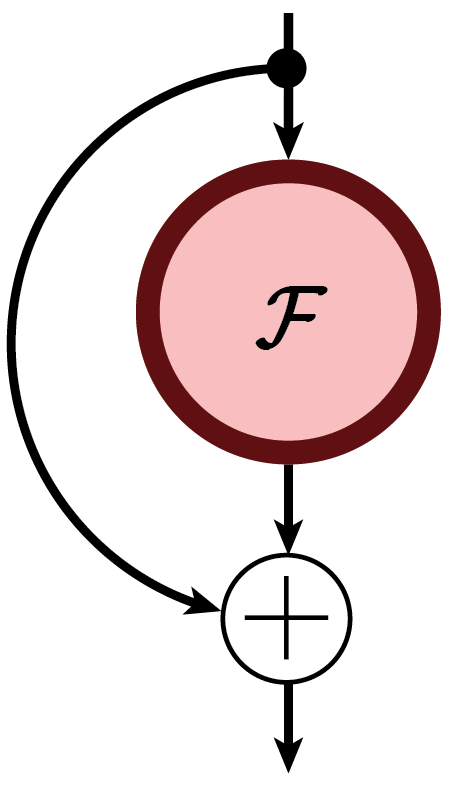
\includegraphics[width=0.13\textwidth]{\imgpath/resnet.png}
  }\qquad
  \subfloat[Lifting]{
  \centering
  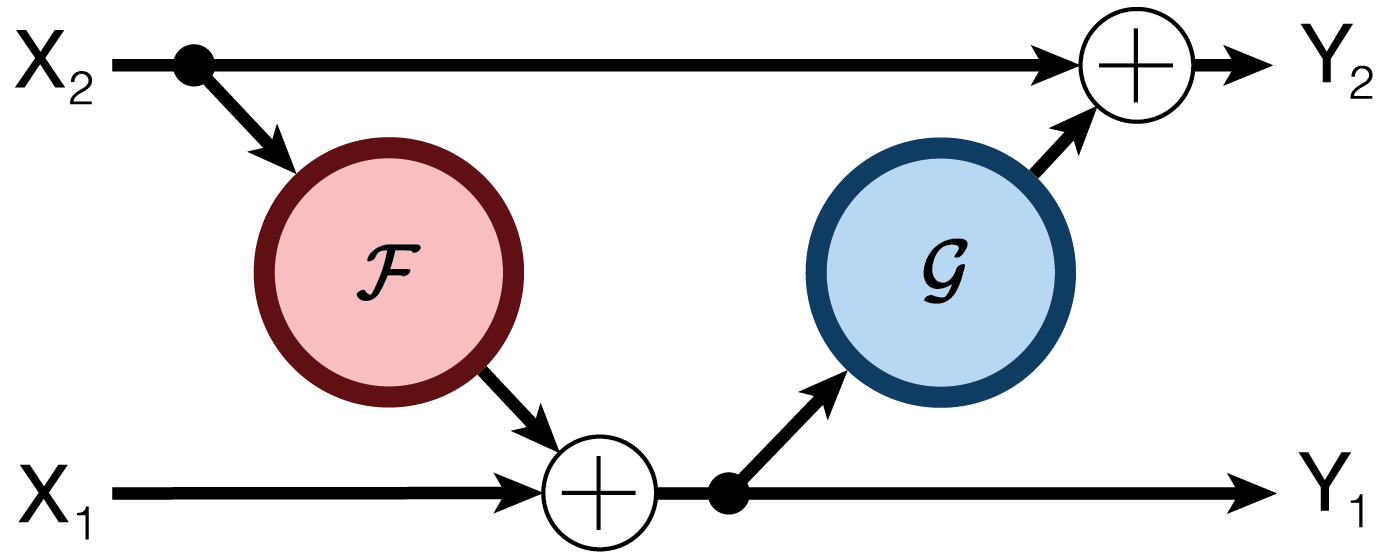
\includegraphics[width=0.48\textwidth]{\imgpath/lifting.png}
  }
  \mycaption{Residual vs lifting layers}{In a residual layer, an input is
  transformed by a learned function $\mathcal{F}$ and added to itself. Typically
  $\norm{\mathcal{F}x} \ll \norm{x}$ meaning the vector $y$ is a small
  perturbation of the vector $x$. In a lifting layer, each path is a learned
  function of the other added to itself. In the original second generation
  wavelets, $\mathcal{F}$ and $\mathcal{G}$ are FIR filters, but there is no
  requirement on them to be. Diagrams are taken from \cite{gomez_reversible_2017}.}
  \label{fig:ch7:lifting_resnet}
\end{figure}

We briefly mentioned ResNets in \autoref{sec:ch2:resnets} but did not study them
in depth in this thesis. Interestingly, there are many similarities between
ResNets and second generation wavelets, or the \emph{lifting} framework
\cite{sweldens_lifting_1998,daubechies_factoring_1998}.
In a residual layer, the output is $y = \mathcal{F}(x) + x$ where for a lifting
system, the layer is a two-port network defined by:
\begin{align}
  y_1 &= \mathcal{F}(x_1) + x_2 \\
  y_2 &= \mathcal{G}(y_1) + x_1
\end{align}
\autoref{fig:ch7:lifting_resnet} shows the similarities between the two designs.
The works \cite{gomez_reversible_2017, jacobsen_i-revnet:_2018} both make the small modifications
to the ResNet design to make a lifting style architecture.
\citeauthor{gomez_reversible_2017} \cite{gomez_reversible_2017} do this to save
memory on the activations for backpropagation (you do not need to save
meta-information on the forward pass as you can regenerate activations on the
backwards pass).
\citeauthor{jacobsen_i-revnet:_2018} \cite{jacobsen_i-revnet:_2018} extend on
\cite{gomez_reversible_2017} and also explore merging images with linear
interpolation in the activation space, reconstructing from the new latent
values. We believe that there are potentially many more benefits to using the
lifting design as an extension of our work into learning from basis functions.

\subsection{Protecting against Attacks}
\begin{figure}
  \centering
  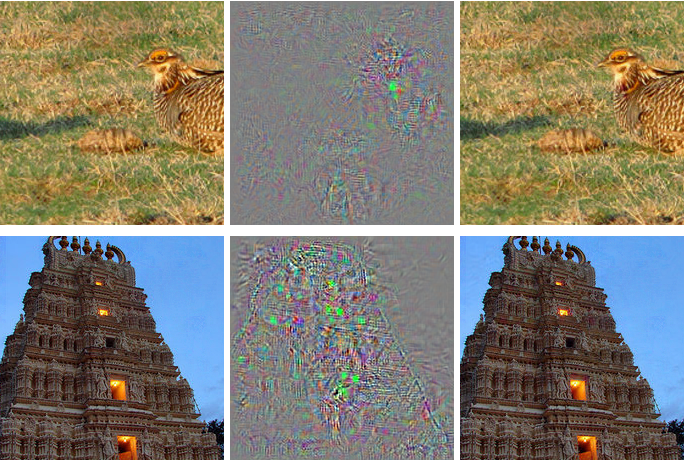
\includegraphics[width=0.8\textwidth]{\imgpath/negative2.png}
  \mycaption{Adversarial examples that can fool AlexNet}{Two examples of images
  that were correctly classified on the left, with additive signals in the
  centre (contrast levels were magnified by 10) and the resulting images on the right. Both of the output
  images are then predicted to be an ostrich. Images are taken from
  \cite{szegedy_intriguing_2014}.}
  \label{fig:ch7:adversarial}
\end{figure}
Adversarial examples are starting to become a real concern for CNNs. A classic
adversarial example is an image that appears innocuous to a human but has been
corrupted with a low energy signal that can completely convince a CNN that the
image is something else. \autoref{fig:ch7:adversarial} shows an example of this
taken from \cite{szegedy_intriguing_2014}.

While \citeauthor{szegedy_intriguing_2014} \cite{szegedy_intriguing_2014} show
there is a weakness to CNNs being fooled, these adversarial examples were
obtained by gradient ascent to the target class. I.e. they had full access to
the parameters of the model. \citeauthor{papernot_practical_2017} \cite{papernot_practical_2017} expand this to show
it is possible to develop an attack without knowing the model, treating it as a
\emph{black box}. Protecting against these black box attacks has become an
arms race in recent years, with measures and counter-measures constantly
being developed. An excellent paper reviewing some attacks and
defences is \cite{carlini_adversarial_2017}.

One such concerning black box attack is described in \cite{engstrom_rotation_2017}, where
\citeauthor{engstrom_rotation_2017} show that even simple transformations such
as translations and rotations are enough to fool many modern CNNs. This is
something our invariant layer may be able to protect against.

Alternatively, a recent defence tactic is described in \cite{cisse_parseval_2017}. In
this paper, \citeauthor{cisse_parseval_2017} propose to have non-expansive
convolutional and pooling layers (Lipschitz constant 1) and have weight matrices
that are approximately Parseval tight frames, a result intimately related to
the tight framed $\DTCWT$. In addition to finding these
networks more robust to adversarial examples, they show that they can train
faster and have a better usage of the capacity of the networks.

We feel that the learning of relatively smooth functions offered by wavelet bases has a potentially
large scope for making CNNs more robust to many attacks.

\subsection{Convolutional Sparse Coding}
Recent work on convolutional sparse coding and convolutional
dictionary learning \cite{liu_online_2017, liu_first_2018,
papyan_convolutional_2017-1, papyan_convolutional_2017, papyan_theoretical_2018}
has started to draw many parallels between the
structure of modern CNN architectures and the problem of sparse
representations. We believe this is a valuable insight and can give a fresh new
perspective on how we can better train CNNs.

It would be interesting to try to extend this recent work on
convolutional sparse coding to wavelet bases. In \cite{rubinstein_double_2010}
\citeauthor{rubinstein_double_2010} attempted something similar with their
double sparsity model, learning to sparsely combine atoms from a fixed base
dictionary (they use wavelet, Fourier and DCT base dictionaries), although this
was applied to block coding and has not been extended to convolutional sparse coding.

\subsection{Weight Matrix Properties}
Some recent work by \citeauthor{advani_high-dimensional_2017}
\cite{advani_high-dimensional_2017} show that if you ignore the
nonlinearities in a neural network, you can analyze the convergence properties
by looking at the conditioning of the weight matrix (the ratio of the largest to
the smallest singular values). In particular, well conditioned matrices have
better convergence, and the size of the \emph{eigengap} (distance between the
smallest non-zero eigenvalue and 0) is important to protect against overfitting.

This is something that we have not enforced or considered in the design of our
wavelet-based layers, and it would be an interesting extension.

% \citeauthor{balestriero_mad_2018} \cite{balestriero_mad_2018} have a related
% view. They view deep neural networks as spline functions, compositions of linear
% mappings and spline points. The underlying intuition behind this is that if an
% input change is small enough, no ReLUs will change state and then the network
% has a linear mapping and transfer function. The Combining this allows for a new
% perspective on deep learning, and it would be an interesting task to try to
% structure any wavelet based layers as well conditioned
\section{Final Remarks}

It is our intuition that complex wavelets in a ScatterNet style system perform well in
CNNs at locations where we want to reduce the sample rate, as they can nicely
demodulate regions of the frequency space to lower frequencies. We also believe
that using complex wavelets without taking the complex modulus is beneficial at
locations where we want filters with large spatial support, something that
is particularly useful in the early layers of CNNs. However, the current trend
in CNNs is shifting away from these uses. Modern architectures typically build
many layers with very small spatial support filters (usually $3\x 3$ and often
$1\x 1$) and lots of mixing and combining of the channels. For example, the
recent Wide ResNet \cite{zagoruyko_wide_2016} (one of the best modern methods),
has close to 1000 channels in the later layers.

We believe that the work in this thesis has opened up a rich vein of ideas and a
new perspective on modern CNN methods. We have found there to be some
performance advantages to redesigning CNNs with complex wavelets as well as
other, less measurable advantages, such as the ability to determine that certain
orientations and frequency regions are less important than others (see
\autoref{sec:ch4:occlusion_results} and \autoref{sec:ch6:analysis}) or the
ability to have smooth roll-of in the support of filters. There is still much
more work to be done; the learning efficiency of CNNs must be improved, as well
as a greater understanding of their operation and outputs if they are to be
widely used in the future.

